\documentclass[../template]{subfiles}

\begin{document}
\section{Flusso a costo minimo}
\begin{center}
    \begin{tikzpicture}[rotate=90, EdgeStyle/.style={->}]
        \Vertices[unit = 2]{circle} {1, 2, 3, 4, 5}
        \Edge[label=$5/9$](1)(2)
        \Edge[label=$15/4$](1)(4)
        \Edge[label=$2/3$](1)(3)
        \Edge[label=$3/11$](2)(4)
        \Edge[label=$2/4$](3)(4)
        ;
    \end{tikzpicture}
\end{center}
\subsection{Classificazione dei nodi}
Nei problemi di flusso a costo minimo, i nodi sono divisi in tre categorie, in base a $b_i$:
\begin{enumerate}
    \item Nodi sorgente: $b_i > 0$, in essi viene realizzato il prodotto.
    \item Nodi di transito: $b_i = 0$, il prodotto transita, senza variazioni
    \item Nodi destinazione: $b_i < 0$, dove il prodotto viene consumato.
\end{enumerate}
La proprietà $\sum_i^n b_i = 0$, quando non risulta valida, è forzabile aggiungendo un fittizio
con $b_{n+1} = -\sum_i^n b_i$, collegato a tutti i nodi sorgente, attraverso archi di costo 0 e capacità $+\infty$.

\subsubsection{Nel caso di archi con capacità illimitata}
\begin{wrapfigure}{R}{0pt}
    \centering
    \begin{tikzpicture}[rotate=90, EdgeStyle/.style={->}]
        \Vertices[unit=1.5]{circle}{1, 2, 3, 4, 5}
        \Edge[label=$5$, color=gray](1)(2)
        \Edge[label=$-2$, color=gray](1)(3)
        \Edge[label=$2$, color=red](1)(5)
        \Edge[label=$-4$, color=red](2)(3)
        \Edge[label=$0$, color=red](3)(4)
        \Edge[label=$6$, color=gray](4)(2)
        \Edge[label=$3$, color=red](4)(5)
        \Edge[label=$4$, color=gray](5)(3)
        ;
        \node[draw] at ([shift={(0:.7cm)}]1)   {$b=2$};
        \node[draw] at ([shift={(0:.7cm)}]2)   {$b=5$};
        \node[draw] at ([shift={(180:.7cm)}]3) {$b=1$};
        \node[draw] at ([shift={(180:.7cm)}]4) {$b=-4$};
        \node[draw] at ([shift={(0:.7cm)}]5)   {$b=-4$};
    \end{tikzpicture}
    \caption{$b_i$ sono indicati vicino al nodo}
    \label{graph:infty_flux}
\end{wrapfigure}
In un problema di flusso su rete a costo minimo una \textbf{base} coincide con un albero di supporto.
Ad ogni base è associabile una soluzione di base, ottenuta ponendo a 0 il flusso (quantità di
prodotto inviata) su tutti gli archi che non fanno parte della base.

\vspace{10pt}
Nell'esempio in figura \ref{graph:infty_flux} prendiamo come esempio la base $B_0 = \{\}$.
Prendiamo come esempio nella rete $G = (V, A)$ in figura \ref{graph:infty_flux}, la
base $B_0 = \{(1, 5), (2, 3), (3, 4), (4, 5)\}$ se poniamo nullo il flusso degli archi
non appartenenti alla base.
Di conseguenza, otteniamo che i flussi relativi agli archi sono:

\vspace{10pt}
\begin{tabular}{cc}
    (1, 5) = &2\\
    (2, 3) = &5\\
    (3, 4) = &6\\
    (4, 5) = &2
\end{tabular}
\\[10pt]
Se i flussi agli archi in base hanno valore non negativo,
\\
allora la soluzione è ammissibile, inoltre se i flussi sono tutti strettamente
maggiore di 0, allora si parla di soluzione non degenere.
Il costo totale di trasporto si calcola semplicemente sommando per ogni arco il prodotto tra
quantità di flusso e costo di trasporto. Nel caso di esempio:
\[
    c_{15} x_{15} + c_{23} x_{23} + c_{34} x_{34} + c_{45} x_{45} =
    2 \cdot 2 - 4 \cdot 5 + 0 \cdot 6 + 3 \cdot 2 = 10
\]
NOTA: questa è solo una possibile soluzione, per sapere se è ottimale occorre confrontarla con
le altre possibili soluzioni al problema.
\subsection{Coefficienti di costo ridotto}
I coefficienti a costo ridotto sono valori numerici associati agli archi che non fanno parte della
base, misurano la variazione del costo di trasporto al crescere dell'unità del valore del flusso
associato tale arco.

\subsubsection{Condizione di ottimalità}
Se i coefficienti di costo ridotto di tutti gli archi fuori base sono non negativi, questo indica che
la crescita del flusso su qualsiasi arco fuori base comporta una crescita del costo di trasporto o
nessuna variazione.
\\
In tal caso possiamo concludere che la soluzione di base attuale è ottima.
Inoltre se tutti i coefficienti a costo ridotto sono strettamente positivi, la soluzione è unica.

\subsubsection{Calcolo dei coefficienti a costo ridotto}
Per calcolare il coefficiente relativo ad un arco fuori base, si aggiunge tale arco alla base attuale,
considerare l'unico ciclo che si forma con tale aggiunta.
Percorrendo il ciclo che si forma nel verso indicato dall'arco, sommo tutti i costi relativi agli archi
percorsi in senso concorde e sottraggo tutti i costi relativi agli archi percorsi in senso opposto.

\subsubsection{Condizione di illimitatezza}
Insieme alla condizione di ottimalità, esiste una seconda condizione d'arresto per l'algoritmo,
che si verifica, quando, l'aggiunta di un arco (alla base) con coefficiente di costo ridotto negativo
forma un ciclo orientato.
\\
La motivazione è facilmente intuibile, siccome il costo di trasporto diminuisce indefinitivamente.

\subsubsection{Dimostrazione}
Dato un flusso ammissibile $\{\bar{x}_{ij}\}$ corrispondente ad una certa base e con valore dell'obbiettivo
(costo di trasporto) $C$.
\\
Sia $\bar{c}_{rs} < 0$ il coefficiente di costo ridotto dell'arco fuori base $(r, s)$.
\\
Sia $r \to s \to l_1 \to \dots l_t \to r$ il ciclo orientato creato aggiungendo alla base l'arco $(r, s)$

Per ogni $\Delta \ge 0$ il seguente aggiornamento del flusso lungo gli archi del ciclo orientato dà origine
ad un flusso ancora ammissibile, con obbiettivo di corrispondenza:
\[
    C + \Delta c_{rs} \to -\infty \quad \text{per}\,\, \Delta \to +\infty
\]
Il che mostra come l'obbiettivo diverga a $-\infty$ sulla regione ammissibile.
\subsection{Cambio di Base}
Nel caso in cui la base scelta non rispetti ne la condizione di ottimalità ne la condizione di illimitatezza
esiste un algoritmo per cambiare la base attuale in una ammissibile.

Scelgo l'arco fuori base con coefficiente di costo ridotto negativo \footnote{Ne esiste almeno uno altrimenti
sarebbe stata soddisfatta la condizione di ottimalità} attraverso un approccio greedy, prendendo quello con
coefficiente di costo ridotto minore, e chiamo tale coefficiente $\bar{c}$.
Aggiungendo tale arco alla base, formando un ciclo.
Tra tutti gli archi percorsi in verso opposto, rimuovo quello con quantità di prodotto su arco minore, e chiamo
tale quantità $-\Delta$. Successivamente, assegno all'arco appena aggiunto una quantità di prodotto inviata
pari a $\Delta$ ed aggiorno il flusso degli archi rimanenti dell'ex-ciclo.

Il nuovo costo è il costo precedente,
Chiamato $T$ il costo precedente, avremo che il nuovo costo sarà dato dalla formula $T + \bar{c} \cdot \Delta$.

\subsection{Algoritmo del simplesso su rete} % Rewrite this subsection better
Dopo aver trovato una base, ripete iterativamente
\begin{enumerate}
    \item Condizione di illimitatezza
    \item condizione di ottimalità
    \item cambio di base
\end{enumerate}
Si può notare che nel caso degenere può cambiare la base, tenendo costante il trasporto e la soluzione di base.
\subsubsection{Problema di 1\textsuperscript{a} fase}
%58
Se il valore ottimo, risultato dalla 1\textsuperscript{a} fase, è maggiore di 0, allora il problema originario ha regione
ammissibile vuota (non ha soluzione).
Se il valore ottimo è uguale a 0, il problema originario ha regione ammissibile non vuota (ha soluzione).
Questo è dovuto al fatto che tutti gli archi di collegamento a $q$, hanno costo 1, mentre quelli del
grafo originario hanno costo nullo. Un valore ottimo nullo, indica che esiste una soluzione all'interno del
grafo originario.

Inoltre, in tal caso esiste un albero di supporto ottimo che contiene solo uno dei nuovi archi (incidenti su $q$).
Eliminando tale arco si ottiene una base ammissibile per il problema originario.
\lstinputlisting{algorithms/unlimited_symplex.py}
\end{document}
